\section{Caso 1. Consultas de una fuente de datos a una ontología}
\label{section:caso1}


Aquí se pretende dar una demostración de cómo realizar una consulta simple a una fuente de datos y una ontología. Para esto se utilizó la Ontología OCDS y los datos de la DNCP. La consulta consiste en obtener de la base de datos toda la información referente a un proceso licitatorio, específicamente el proceso cuyo identificacor es <http://www.contrataciones.gov.py/datos/api/v2/doc/release/302438-adquisicion-semillas-gdc-1>, ya que es un Proceso Licitatorio que contemple las fases de Planificación, Convocatoria, Adjudicación y Contratación.

En el Cuadro \ref{lst:caso1} se muestra la consulta realizada al Punto SPARQL.

\noindent\begin{minipage}[t]{\textwidth}
\begin{lstlisting}[captionpos=b, caption={Tripas referentes al proceso licitatorio cuyo identificador es 302438}, label={lst:caso1},  numbers=left,  numberstyle=\tiny\color{mygray},frame=single]
SELECT *  
WHERE {    	
    <http://www.cont...e/302438-adquisicion-semillas-gdc-1> rdf:type ocds:Release .
    <http://www.cont...ase/302438-adquisicion-semillas-gdc-1> ?propiedadNivel1 ?recursoNivel1 .   
    OPTIONAL { ?recursoNivel1 ?propiedadNivel2 ?recursoNivel2}
}  
 \end{lstlisting}
\end{minipage}

 Si se considera el resultado de esta consulta un árbol, donde la raíz es el Proceso Licitatorio, entonces la consulta traerá la información del proceso licitatorio hasta el segundo nivel del árbol. En la figura \ref{img:caso1Diagrama} se muestra gráficamente el resultado de la consulta. Aquí se puede ver que el único valor literal obtenido en el nivel 1 es "ocds:ReleaseTag", los demás nodos representan un identificador a un nuevo recursos que podrán ser accedidos en el segundo nivel del árbol.
 
 \begin{figure}[ht!]
    \centering
    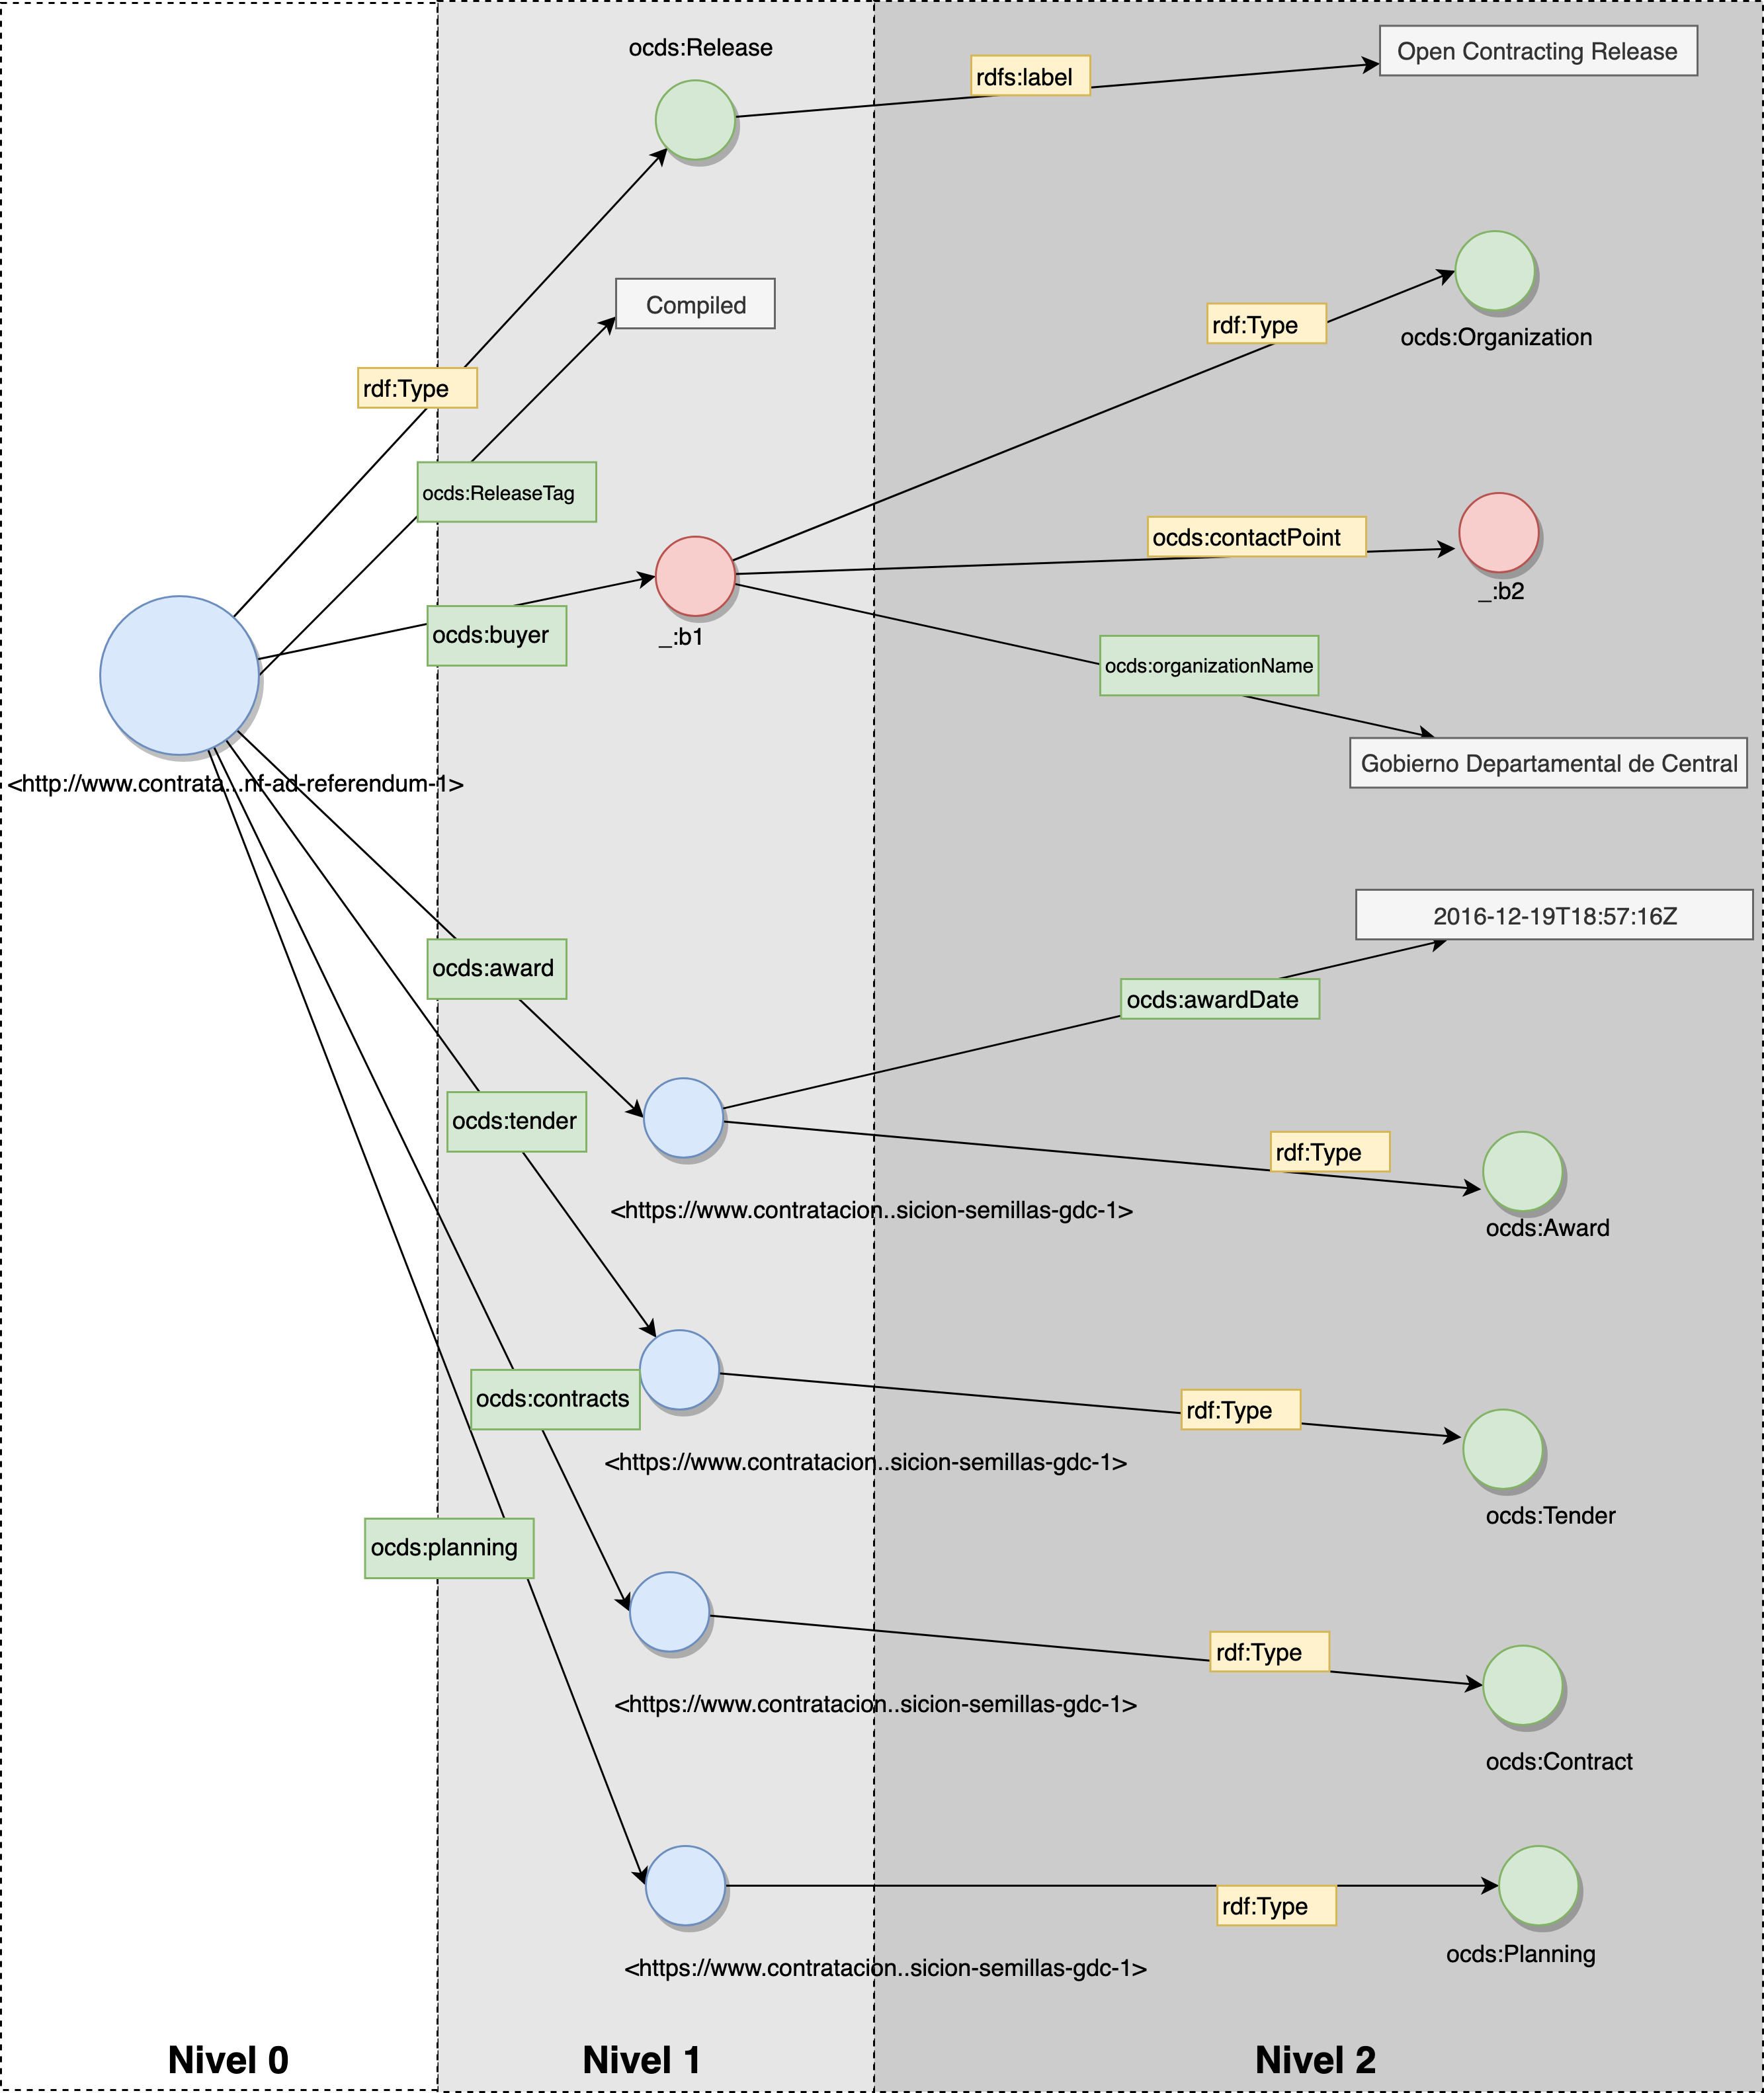
\includegraphics[width=150mm]{figuras/Diagramas-Caso1.png}
    \caption{Árbol de información de la consulta del caso 1}
    \label{img:caso1Diagrama}
 \end{figure}

En la Figura \ref{img:caso1Resultado} se muestran los resultados obtenidos. Los nodos de un nivel representan un recurso o un literal. Se puede observar que el resultado contiene tanto los datos propios del Proceso de Contratación, agrupado a traves del concepto "ocds:Release", como es “ocds:ReleaseTag” cuyo valor es “compiled” y también contiene datos del Comprador (ocds:buyer) del bien o servicio como puede ser el nombre de la organización oferente (ocds:organizationName) cuyo valor es “Gobierno Departamental de Central”. El valor “compiled” fue posible obtener a partir de la sentencia de la línea 4 y el valor “Gobierno Departamental de Central” a partir de la sentencia de la línea 5.

En la línea 3 del Cuadro \ref{lst:caso1} encontramos la restricción cuya intención es asegurar que el recurso se trate de un Release, esto es posible debido a la utilización de la ontología desarrollada. En la línea 4 se consulta por el conjunto de triplas que cumplan la condición de tener como sujeto la URI del proceso licitatorio, osea el primer nivel del árbol. Con la sentencia de la línea 5 se obtienen las triplas que tengan como sujeto el objeto proveniente del resultado de la primera sentencia. En otras otras palabras, se obtienen datos provenientes del segundo nivel del árbol. Haciendo esta segunda sentencia opcional, se puede también desplegar aquellas triplas que no tienen un segundo nivel en el árbol, por ende se muestran los datos directos del Proceso Licitatorio.

En este caso se muestran las siguientes mejoras de trabajar con triplas RDF y ontologías. L ontontologias son xxlksandf agrandara kajsndfkjlnasdxxxx

\subsection{Mejora 1: Consultas sin conocer las propiedades del concepto}

Podemos ver en el Cuadro \ref{lst:caso1}, que no es necesario conocer las propiedades, tipos de datos ni relaciones existentes entre los conceptos para realizar la consulta, es decir nos permite realizar consultas donde el modelo de datos no es necesariamente conocido. El único dato necesario fue la URI de un Proceso de Contratación. En cambio, si comparamos con una consulta en una base de datos relacional, para obtener todos los datos de un Proceso de Contratación, se requeriría realizar un JOIN entre varias tablas relacionadas.  Para poder realizar esto necesitaríamos conocer cuáles son las tablas involucradas y cuáles son las columnas para aplicar el JOIN correctamente En este caso, un JOIN con la tabla del Planificación, Convocatoria, Adjudicación, Contrato  y el Proceso de  Contratación en sí.

\subsection{Mejora 2: Nivel de granularidad de la información}

A diferencia de una consulta a una API REST tradicional, gracias a SPARQL podemos elegir hasta qué grado de detalle de datos mostrar. Agregando una linea de código más, se podría extender la granularidad de los datos al tercer nivel y así sucesivamente, o elegir específicamente qué rama del árbol expandir.

\subsection{Mejora 3: Semántica de los nodos y sus relaciones}

Como el grafo está enriquecido por una ontología, se puede extraer el significado de cada uno de los objetos, como ejemplo, sabemos que el nodo ":b01" de la Figura \ref{img:caso1Diagrama} es de tipo "ocds:Organization", por lo tanto corresponde a una organización, y la relación entre el proceso licitatorio y la organización es de tipo "ocds:buyer", por lo que se puede decir que la organización a la que se refiere es la organización compradora del producto o servicio. De otra manara, no habría forma que un sistema computacional entienda el significado de los nodos y su relación entre ambos .
    

\begin{figure}[ht!]
    \centering
    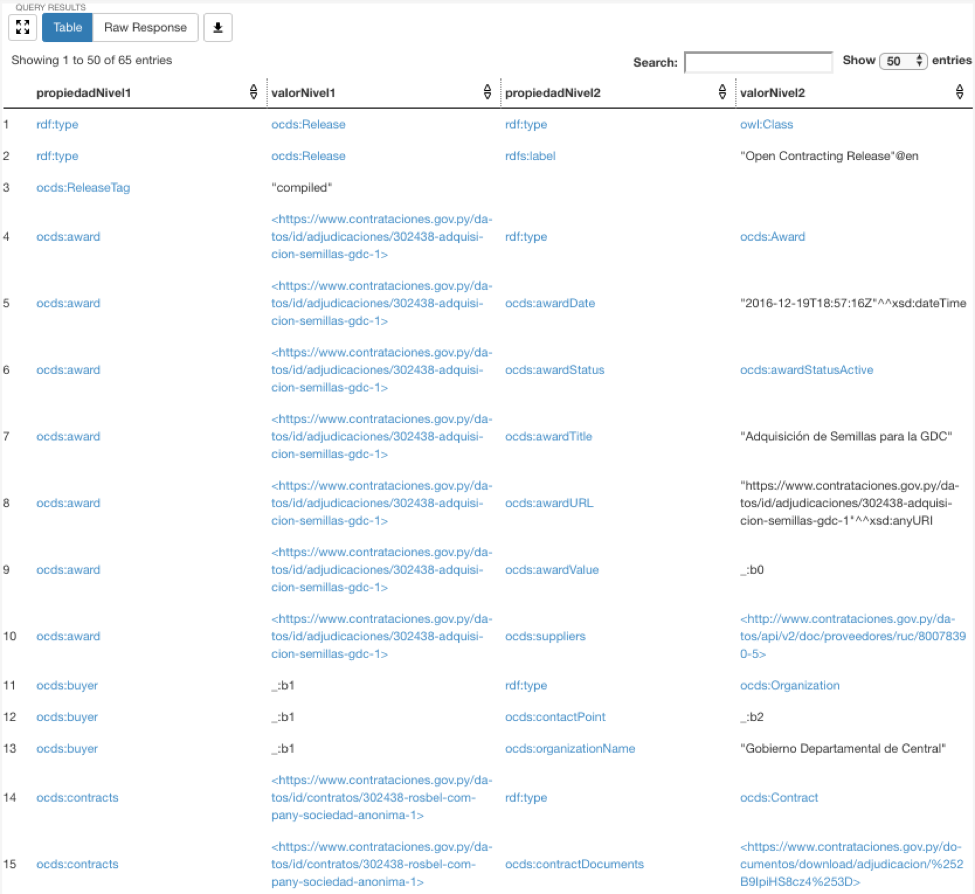
\includegraphics[width=150mm]{figuras/caso1Resultado.png}
    \caption{Despliegue de resultado de la consulta de l caso 1}
    \label{img:caso1Resultado}
 \end{figure}
